\chapter{TINJAUAN PUSTAKA}
\section{Teori Dasar}
  \subsection{Arsitektur Famili YOLO}
    Arsitektur famili YOLO pada dasarnya terbagi akan 3 bagian yaitu \emph{head}, \emph{neck}, dan \emph{backbone}.
    Setiap bagian ini mempunyai fungsi masing-masing.
    Berikut adalah penjelasan fungsi dan cara kerja dari ketiga bagian tersebut.
    \subsubsection{\emph{Layer Head} YOLO dan \emph{Anchor Box}}
      \begin{figure}[H]
          \centering
          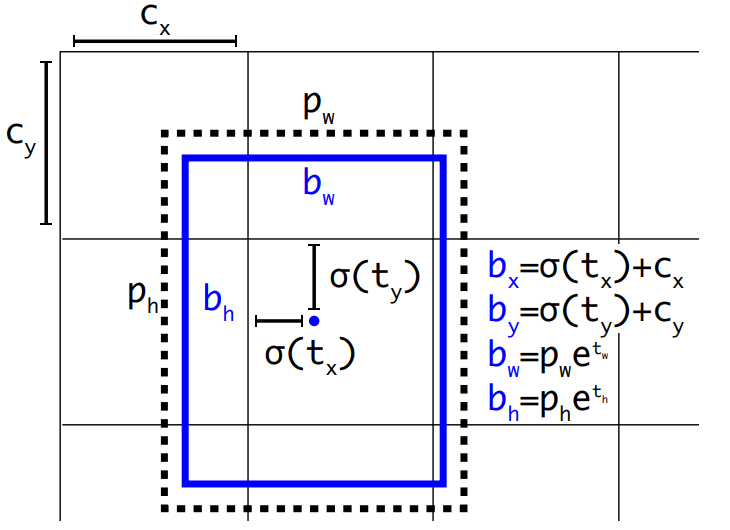
\includegraphics[scale=0.4]{figures/anchorbox.png}
          \caption{Prediksi \emph{Anchor Box} dan \emph{offset} dari koordinat latis \parencite{yolov3}}
          \label{fig:anchorbox}
      \end{figure}
      Arsitektur famili YOLO yang dipublikasikan setelah YOLOv2 terus menggunakan \emph{anchor box} untuk melakukan deteksi \parencites{yolov2}{yolov3}{yolov4}{scaledyolov4}{yolov5}{yolor}{yolov7}.
      \emph{Anchor boxes} merupakan beberapa \emph{Bounding Box} yang telah terdefinisikan. 
      Arsitektur YOLO akan memprediksi probabilitas \emph{anchor box} berada pada suatu koordinat latis beserta dengan \emph{offset anchor box} tersebut untuk menepatkan \emph{anchor box} pada objek yang dideteksi.
      Penggunaan \emph{anchor box} ini dapat meningkatkan akurasi deteksi karena \emph{neural network} hanya perlu mencari titik tengah objek dan \emph{error} dimensi \emph{boudning box} dengan menggunakan \emph{offset} \parencite{yolov3}.
      Hal ini lebih sederhana daripada mencari titik-titik \emph{bounding box} secara independen sehingga lebih mudah untuk dipelajari oleh \emph{neural network}.
  
      Prediksi \emph{bounding boxes} terjadi di bagian \emph{head} dari arsitektur YOLO.
      Bagian \emph{head} dari YOLO akan mengambil beberapa hasil \emph{upsampling} yang terjadi pada \emph{neck} YOLO, dan kemudian melakukan prediksi \emph{anchor boxes} dari hasil tersebut.
      Hasil prediksi \emph{Head} YOLO pada suatu tingkatan \emph{upsampling} berupa tensor dengan ukuran $N\times N \times [A\times(4+1+C)]$ dengan $N$ sebagai dimensi hasil \emph{upsampling}-nya, $A$ sebagai jumlah \emph{anchor boxes} untuk \emph{scaling} tersebut, dan $C$ sebagai jumlah kelas prediksi.
      Angka 4 merepresentasikan 4 \emph{offset} $b_x, b_y, b_w, b_h$ seperti pada Gambar \ref{fig:anchorbox} dan angka 1 merepresentasikan \emph{objectness score} dari prediksi \emph{bounding box}.
  
    \subsubsection{\emph{Neck} YOLO}
  
      \begin{figure}[H]
          \centering
          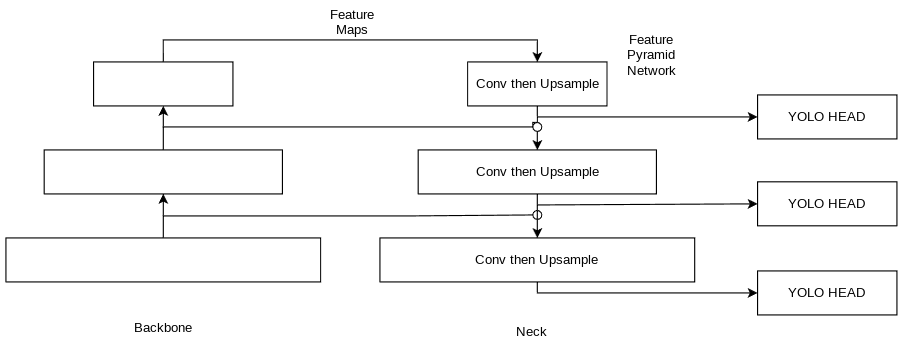
\includegraphics[scale=0.6]{figures/yolo-architecture-rough.png}
          \caption{\emph{Feature Pyramid Network} pada \emph{Neck} YOLO}
          \label{fig:yolofpn}
      \end{figure}
  
      \emph{Neck} dari YOLO merupakan \emph{layer-layer} dimana \emph{head} YOLO mengambil fitur untuk dilakukan deteksi \emph{bounding box}.
      Pada YOLOv3 \textcite{yolov3}, arsitektur \emph{neck} dibuat menyerupai \emph{Feature Pyramid Network} (FPN) seperti pada Gambar \ref{fig:yolofpn}. 
      Pada versi-versi YOLO selanjutnya, bentuk \emph{neck} ini tidak banyak berubah dan pada dasarnya tetap mempertahankan bentuk \emph{pyramid}-nya.
  
      Penaikkan tingkatan \emph{pyramid} dari FPN merupakan \emph{upsampling} dari \emph{feature map} yang dihasilkan \emph{backbone}.
      Output tiap tingkatan pada FPN di \emph{neck} inilah yang diinputkan pada \emph{head} YOLO. 
      Melakukan prediksi pada tingkatan \emph{upsampling} yang berbeda-beda dapat membuat \emph{neural network} mendapatkan lebih banyak informasi semantik dan informasi yang lebih detail sehingga dapat lebih akurat dalam mendeteksi objek besar maupun kecil.
  
    \subsubsection{\emph{Backbone} YOLO}
      \emph{Backbone} dari YOLO merupakan bagian yang mengekstrak fitur dari citra yang diinputkan.
      Hasil ekstraksi fitur ini akan diinputkan pada \emph{neck} yang kemudian akan di\emph{upsampling} olehnya.
      Model-model YOLO dapat menggunakan \emph{feature extractor} dari model-model klasifikasi citra sebagai \emph{backbone}-nya.
      Sebagai contoh, salah satu varian YOLO, YOLO-Z menggunakan DenseNet sebagai \emph{backbone}-nya sedangkan arsitektur YOLO dasarnya, YOLOv5 menggunakan \emph{backbone} YOLOv5v7.0 \parencite{yoloz}.
  
  
  
  
  \subsection{YOLOv7}
    YOLOv7 merupakan pendeteksi objek \emph{real time} dengan skor akurasi tertinggi pada dataset COCO di tahun 2022.
    Pada YOLOv7, dilakukan beberapa perubahan untuk meningkatkan akurasi dan kecepatan deteksinya.
    Perubahan-perubahan tersebut dilakukan pada arsitekturnya dan pada \emph{bag-of-freebies}-nya.
  
    Perubahan arsitektur dilakukan pada \emph{backbone}. YOLOv7 menggunakan \emph{Extended Efficient Layer Aggregation Network} (E-ELAN) sebagai \emph{backbone}, berbeda dengan leluhurnya YOLOv4 yang menggunakan CSP-Darknet.
    E-ELAN merupakan arsitektur \emph{neural network} yang efisien karena E-ELAN didesain dengan mengontrol \emph{gradient path} terpanjang yang terpendek.
    Karena efisiensinya, arsitektur E-ELAN ini dapat meningkatkan kecepatan deteksi dan akurasi. \parencite{yolov7}
  
    \emph{Bag-of-freebies} merupakan kumpulan metode peningkatan akurasi yang tidak meningkatkan \emph{cost inferrence} \parencite{yolov4}. 
    Pada YOLOv7, ditambahkan beberapa \emph{bag-of-freebies} yang dapat dilatih seperti \emph{re-parameterized convolution} dan \emph{extra auxilary head} di tengah-tengah \emph{neural network}.
    Selain kedua itu, YOLOv7 juga menambahkan \emph{trainable bag-of-freebies} dari YOLOR seperti EMA, \emph{Implicit Knowledge}, dan \emph{conv-bn topology Batch Normalization} \parencite{yolov7}.


\section{Rekalkulasi \emph{Anchor}}
  \emph{Anchor box} dari model-model \emph{pre-trained} YOLO pada umumnya mengoptimisasi \emph{anchor box} modelnya pada dataset COCO.
  Ukuran \emph{anchor box} yang akan digunakan pada model YOLO dapat dikonfigurasikan agar lebih sesuai dengan dataset yang akan digunakan untuk melatih model YOLO.
  Penyesuaian ini dapat meningkatkan IoU(\emph{Intersection Over Union}) prediksi model dengan \emph{ground truth} sehingga meningkatkan akurasi.

  Penyesuaian anchor box dapat dilakukan pada saat sebelum training atau pada saat training.
  Penyesuaian anchor box sebelum training dapat dilakukan dengan cara mengkonfigurasi secara manual tiap ukuran \emph{anchor box} atau dengan menggunakan algoritma \emph{clustering}.
  Penggunaan algoritma \emph{clustering} akan lebih baik karena setiap ukuran \emph{anchor box}-nya disesuaikan dengan pengelompokan-pengelompokan ukuran \emph{bounding box} natural yang terdapat pada dataset.
  Untuk penyesuaian saat training, dapat digunakan algoritma dari \textcite{anchoropt}.
  Algoritma ini akan mengoptimisasi ukuran-ukuran anchor bukan hanya berdasarkan dataset, namun berdasarkan kemampuan dari neural network pendeteksi objeknya.
  Untuk melakukan hal tersebut, algoritma ini akan memanfaatkan back propagation localization loss untuk rekalkulasi anchor.

\section{Augmentasi Mosaik}
\label{section:mosaic_study}
  \begin{figure}[H]
    \centering
    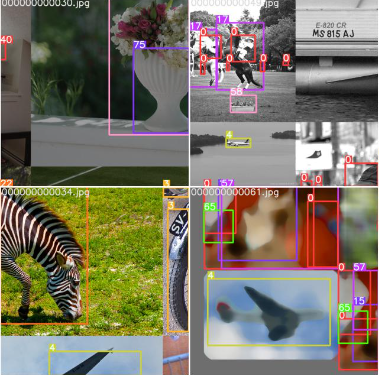
\includegraphics[scale=0.6]{figures/mosaic-aug.png}
    \caption{Contoh Augmentasi Data Mosaik \parencite{yolov5}}
    \label{fig:mosaic}
  \end{figure}

  Augmentasi mosaik merupakan teknik augmentasi yang baru dikenalkan pada YOLOv4.
  Teknik augmentasi ini akan memilih 4 gambar dari dataset, memotong gambar-gambar tersebut dan menggabungkannya secara acak pada satu gambar seperti pada Gambar \ref{fig:mosaic}.
  Hasil dari penggabungan itu membuat gambar terlihat seperti mosaik.
  Teknik augmentasi ini mampu meningkatkan akurasi model \parencite{yolov4}.


\section{Penelitian Terkait}
\label{section:relatedwork}

  \subsection{YOLO-Z}
    YOLO-Z merupakan arsitektur famili YOLO yang modifikasi dari YOLOv5 \parencite{yoloz}.
    Modifikasi-modifikasi yang dilakukan meliputi pergantian \emph{backbone}, \emph{neck}, dan jumlah \emph{anchor}
    \emph{Backbone} dari YOLOv5r5.0 menjadi DenseNet yang di-\emph{downscale}.
    \emph{Neck} dari YOLO-Z juga diganti dari PanNet menjadi FPN dan biFPN tergatung pada \emph{scale} YOLO-Z yang digunakan.

    Modifikasi pada YOLO-Z didesain untuk mendeteksi objek kecil untuk tujuan melakukan deteksi \emph{cone} yang nampak jauh pada lintasan \emph{autonomous racing} secara \emph{real time} (lihat Gambar \ref{fig:yolozcone}).
    Modifikasi-modifikasi dibuktikan dapat meningkatkan kemampuan pendeteksian objek kecil \parencite{yoloz}.
    Oleh karena itu, untuk meningkatkan kemampuan mendeteksi objek kecil YOLOv7, beberapa modifikasi yang dilakukan YOLO-Z pada YOLOv5 dapat diaplikasikan.
    \begin{figure}[H]
      \centering
      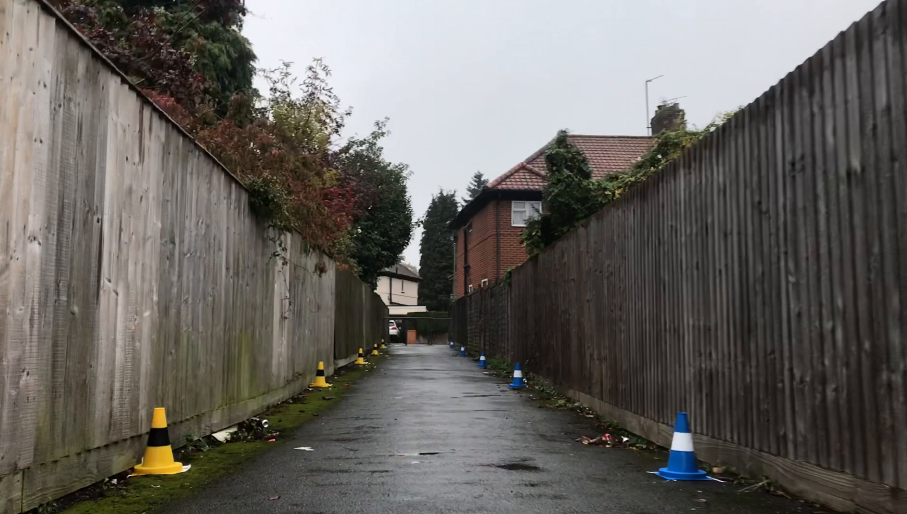
\includegraphics[scale=0.4]{figures/yoloz-cone.png}
      \caption{Contoh Objek \emph{Cone} yang Terlihat Jauh dari Kamera}
      \label{fig:yolozcone}
    \end{figure}

  \subsection{exYOLO}
    exYOLO merupakan hasil modifikasi arsitektur YOLOv3 \parencite{exyolo}.
    Pada exYOLO, dilakukan modifikasi \emph{neck} dengan menambahkan suatu \emph{Receptive Field Block} sebelum penggabungan \emph{feature map} yang akan diupsampling.
    Modifikasi-modifikasi ini membuat exYOLO memiliki skor mAP yang lebih tinggi daripada YOLOv3 pada dataset PASCAL VOC 2007.

  \subsection{Implementasi YOLOv4-tiny pada \emph{Autonomous Surface Vehicle}}
  \textcite{barunastra} menggunakan model modifikasi YOLOv4-tiny pada \emph{Autonomous Surface Vehicle}(ASV) mereka.
  YOLOv4-tiny sebenarnya hanya menggunakan 2 layer head, namun yang diimplementasikan pada ASV adalah model YOLOv4-tiny
  yang ditambahkan 1 layer head lagi sehingga menggunakan total sebanyak 3 layer head. Perubahan ini memberikan peningkatan
  pada skor mAP dan memberikan kemampuan modelnya untuk mendeteksi objek yang lebih jauh.